\documentclass{tufte-handout}
%\documentclass[12pt]{book}
\usepackage{color}
\usepackage{graphicx}
\usepackage{palatino}
\usepackage{mathpazo}
\usepackage{url}
\usepackage{amsmath, amsthm, amssymb}
\usepackage{subfigure}
\newtheorem{del}{Exercise}
\newtheorem{con}{Conjecture}
\newcommand{\beforefig}{\vspace{0.2in}}
\newcommand{\afterfig}{\vspace{0.2in}}


\title{Abstraction, Act 3}

\author{Dynamics of Mechanical Systems}

%\date{Fall 2011}

\begin{document}
\maketitle


\section{Where we're going}

Thus far we've talked about populations (modeling how numbers of organisms change in time) , about thermal systems (modeling how the internal energy and temperature of a system or subsystem changes in time), and about pharmacokinetic systems (modeling how the concentrations of drugs in different parts of the body change in time).

In this section of the course, we're going to do some modeling that probably, at least on the face of it, looks more familiar:  mechanical systems.  If you look up the definition of mechanics, you'll find that it is the study of {\it motion}: how the positions and orientations of physical objects change in time.  So pretty much any time that we're asking questions about how objects move, we're asking mechanics questions.  

\begin{marginfigure}
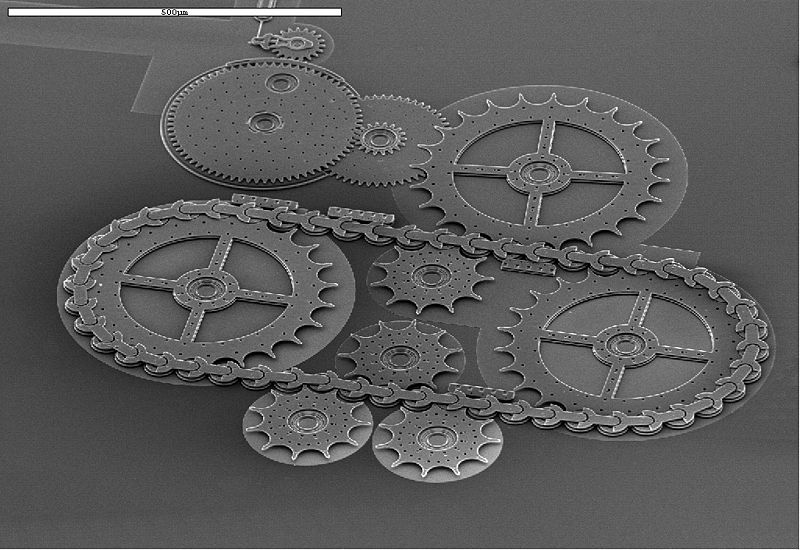
\includegraphics[width=6cm]{figs/MEMS}
\caption{MEMS: A Micro Electro Mechanical System}
\end{marginfigure}

Some mechanics questions are relatively easy to answer.  For example, if you ask about how a cannonball dropped from a high building moves, you can make pretty reasonable predictions using simple models that you are already familiar with.  Other mechanics questions are very difficult indeed:  while bipedal walking is something we do every day, understanding the dynamics of walking is an area of current research. 

You've already dealt with this to a some extent in high school physics.  You've probably seen a number of important ideas, like using a coordinate system to describe where an object is;
describing an object's motion using vectors that descibe the object's position, velocity, and acceleration;
using a free body diagram to represent what forces are acting on the body;
 and using Newton's second law ($\vec{F} = m\vec{a}$) to determine the body's acceleration.  At the same time, it's often the case in high school physics that you start out with an assumed model:  you look at the problem, say, ``A ha!  This is a projectile motion problem!'', and immediately jump to $y = y_0 + v_{y0} t - \frac{1}{2} g t^2$.


In this section of the course, we'll be a little more explicit about {\it abstracting} the model -- i.e., making intentional decisions about what to include, what to ignore,  and how to capture the effects you're interested in.  Typically this will boil down to the following steps:
\begin{enumerate}
\item First you do some qualitative abstraction.  This is a bit like developing a stock-and-flow diagram, or a system diagram:
\begin{enumerate}
\item You first spend some time just {\it thinking about it.}  How do you think the system will behave?  What might or might not be important?
\item Then you identify a {\it system boundary, and subsystem boundaries}:  what are the parts of the {\it system}, and what is the {\it rest of the world}.  Does your system have one piece or multiple pieces?  
\item You identify what {\it characteristics of the system parts} you're including and which you are leaving out of your model: are you building a really simple model, or a more complex model?  Do the pieces of your system rotate?  Translate?    
\item You identify what {\it interactions} you are trying to capture in your model, and which parts of the system they affect.  Are you including gravity?  Friction?  Air drag?
\item You capture this information in a {\it free-body diagram}.  Just as in thermodynamics modeling, you draw a diagram that identifies the system and subsystem boundaries, and how those parts interact with the rest of the system or world. 
\end{enumerate}
\item Then you do more quantitative abstraction:  how are you mathematically going to model the system?
\begin{enumerate}
 \item You develop {\it mathematical models for the interactions}.  How are you modeling the interaction with the ground?  Air drag?  etc.?
\item You define a set of {\it variables and parameters that describe the system}.  In thermodynamic systems, you typically track the internal energies of parts of the system -- and you worry about parameters like thermal conductivity, specific heat, etc.  In modeling the dynamics of mechanical systems, the variables you typically want you need a way to track are the positions, velocities, and angular positions and velocities of the different parts  -- and so you need a coordinate system to define these variables. Typical parameters include mass, moment of inertia, spring constants, etc. 
\item Finally, you combine this work in a set of {\it differential equations} that describe how the variables you're tracking change over time.
\end{enumerate}
\end{enumerate}


\section{Qualitative Abstraction of Mechanical Systems}
One of the really important things in dealing with any modeling problem is deciding how far to take your abstraction -- in other words, what are you going to ignore, and what are you going to include.  Mechanics is no different.   In deciding what you're going to ignore or include, there are some important questions that you can ask...
%\subsection{Where is the boundary?}
% When you draw a stock and flow diagram, or a system diagram in thermo, you are deciding a couple of things.  First, you're deciding what you are going to track, and what you're not going to track: in a population model, if you use a sink for ``dead owls'', you're saying, ''I am not tracking the number of dead owls, and I don't believe the number of dead owls is important''.  Similarly, if you draw a system diagram around a pot that's on a stove, you're saying ``I don't really care what the internal energy of hte stove is -- I only care what the pot's internal energy is.
% 
%Note that this does not mean that you don't care what is {\it happening} outside of the system.  For example, in the case of the pot, you would care if the stove was turned on or not -- but you would talk about this as a power flow across the system boundary.    What it does mean is that you are assuming that, while the stuff outside the system affects the stuff inside the system, the effect of the system on the rest of the world is either too small to be important, or is something you just don't care about.
%
%Similarly, you might care about what the external temperature in the room was -- but rather than assuming that is is controlled 

\subsection{How will it behave?}
As in almost any modeling situation, it's good to think in advance about possible ways that the system might behave -- to ``play the movie in your head''.  Naturally you can't predict every possible behavior of the system, but thinking through possible scenarios in advance helps you identify the things you'll need to take into account in your model.  
\begin{marginfigure}
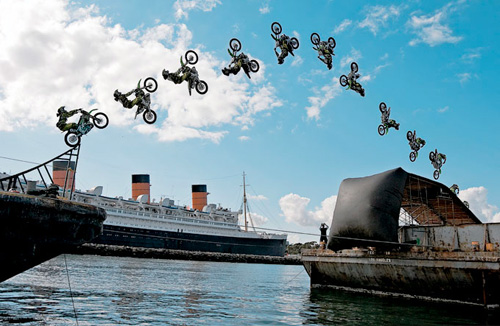
\includegraphics[width=6cm]{figs/motorcyclekeyframe}
\caption{Don't try this at home.  From {\tt http://khalednoorblog.com}
 }
\end{marginfigure}
In the case of mechanical systems, this idea of ``playing the movie in your head'' is particularly helpful, because as humans we are relatively good at intuiting how things move (because it tended to help us get eaten or killed back in the good ol' days).  One good way to do this is to draw a set of keyframes for the system -- show a series of snapshots that show the system at different points in time.

\subsection{One part or many parts?}
Often a mechanical system can be thought of either as consisting of a ``single lump'' or as consisting of multiple subsystems.  For example, if you think about a car, you might say ``I'm going to think about the car as one thing'', or ``I'm going to think about the wheels as distinct from the body of the car'', or ``I am going to worry about how different parts of the engine are moving''.  In the first case, you've abstracted away all of the details about what's going on inside the ``car system''; whereas in the second and third cases you're breaking the system down into more and more parts -- each of which you can ask questions about.

In general, fewer parts is simpler.  That was obvious, wasn't it?

\subsection{Partlcles, rigid bodies, or flexible bodies?}

\begin{marginfigure}
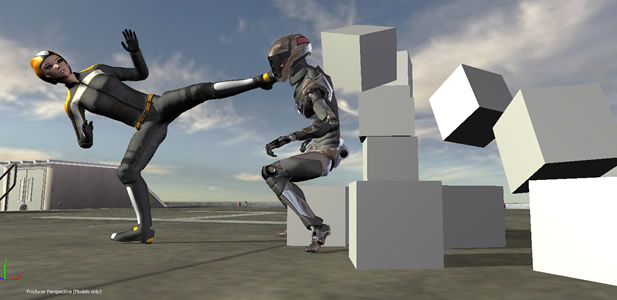
\includegraphics[width=6cm]{figs/rigidbodies}
\caption{Multiple rigid bodies.  From {\tt autodesk.com}
 }
\end{marginfigure}

\begin{marginfigure}
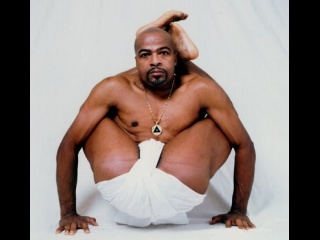
\includegraphics[width=6cm]{figs/flexiblebody}
\caption{One flexible body.  From {\tt http://my.opera.com/Sadiya23}
 }
\end{marginfigure}
You can also make choices about how much information you try to track about an individual part of a system.  You might decide to track just the location of a part (e.g., tracking a ping pong ball's location as it travels across the ping pong table).  Or you might be interested not only in the ball's position, but also in its rotation:  how does its spin change over time?  Or you might even be interested in how the ball's shape changes over time-- maybe, due to being hit by the paddle, it oscillates between being a prolate and an oblate ellipsoid, and perhaps for some reason (don't ask me why) you're interested in building a model that characterizes the behavior.

Generally the simplest option is to treat objects as particles, where you don't care about their orientation or their deformation.  But in lots of real situations, orientation and deformation can be very important.  For the purposes of this class, we're not planning to deal with deformation at all -- but you can, of course, choose to pursue this if you wish.

\subsection{What are the interactions?}
Whether you choose to abstract the parts of the system as particles or as rigid bodies, you also need to think about how these parts are ``connected'' to each other, and to the rest of the universe -- and you need to decide which of these interactions will be important.  Gravity, for example, connects every mass in the universe to every other mass in the universe -- but when you're modeling a bat hitting a baseball, you typically don't worry about the gravitational attraction between the bat and the ball, whereas you do think about the gravitational interaction between the earth and the ball. 

\subsection{What is the graphical representation?}

Just as in the previous cases we've dealt with, it's important to create a visual representation of how you are thinking about the system you're modeling.  For mechanical systems, the canonical representation is the {\it free body diagram}, which shows how you've decided to abstract the system, as well as what interactions you have identified as being important in the system.  

It's worth asking why free body diagrams are so named.  An easy way to think about it is that free body diagrams show each body (part of the system) as if you ``cut it out of the universe'', as well as each of the interactions you had to cut through in order to release the object from the universe.  So if you're modeling a baseball flying through the air, and you've decided that the only important interactions are the gravitational interaction between the ball and the earth and the interaction between the ball and the air it is moving through was also important, you might make a diagram like this:


\centerline{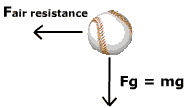
\includegraphics[height=1in]{figs/baseballfbd}
From {\tt eloquentlogic.com}}


\section{An Example of Qualitative Abstraction: The Skateboard Ramp}

To illustrate the ideas thus far, let's walk through these steps for the pivoting skateboard ramp.  In case you don't recall the details of this from the poster, here's the setup:

\begin{quote}
The International Skateboard Federation is considering including
 a new skateboard ramp competition in the next World
Games. Unlike a typical skateboard ramp, this one is free to pivot
about a support point.  Skateboarders approach the ramp on a flat
surface and then coast up the ramp; they are not allowed to put their
feet down while on the ramp.  If they go fast enough, the ramp will
rotate and they will gracefully ride down the rotating ramp.
Technical and artistic display will be assessed by the usual panel of
talented judges.
The Federation has requested a model-based assessment of whether this concept is a good one.

\begin{marginfigure}
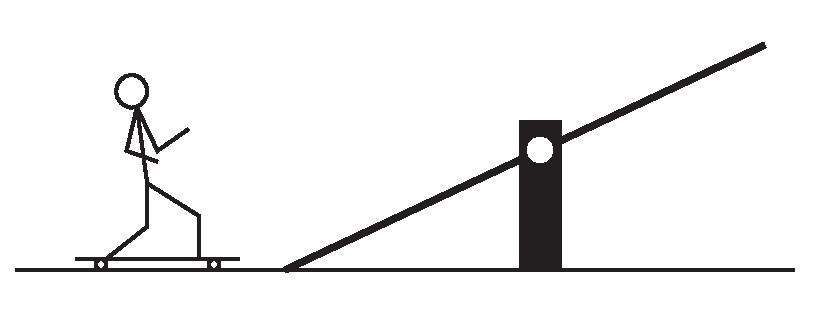
\includegraphics[width=7cm]{figs/skateboard1}
\caption{The proposed stunt setup.}
\end{marginfigure}

\end{quote}

\subsection{How will the skateboard system behave?}

To think about this, we'll try to imagine what some of the keyframes are for the motion of the skateboarder.  A first guess at this is that there are three options for motion:  first, the skateboarder could be going so slowly that they don't make it over.  Second, the skateboarder could be going at just the right speed to have the ramp land, and allow a smooth exit.  And finally, the skateboarder could be so fast that they fly off the ramp.

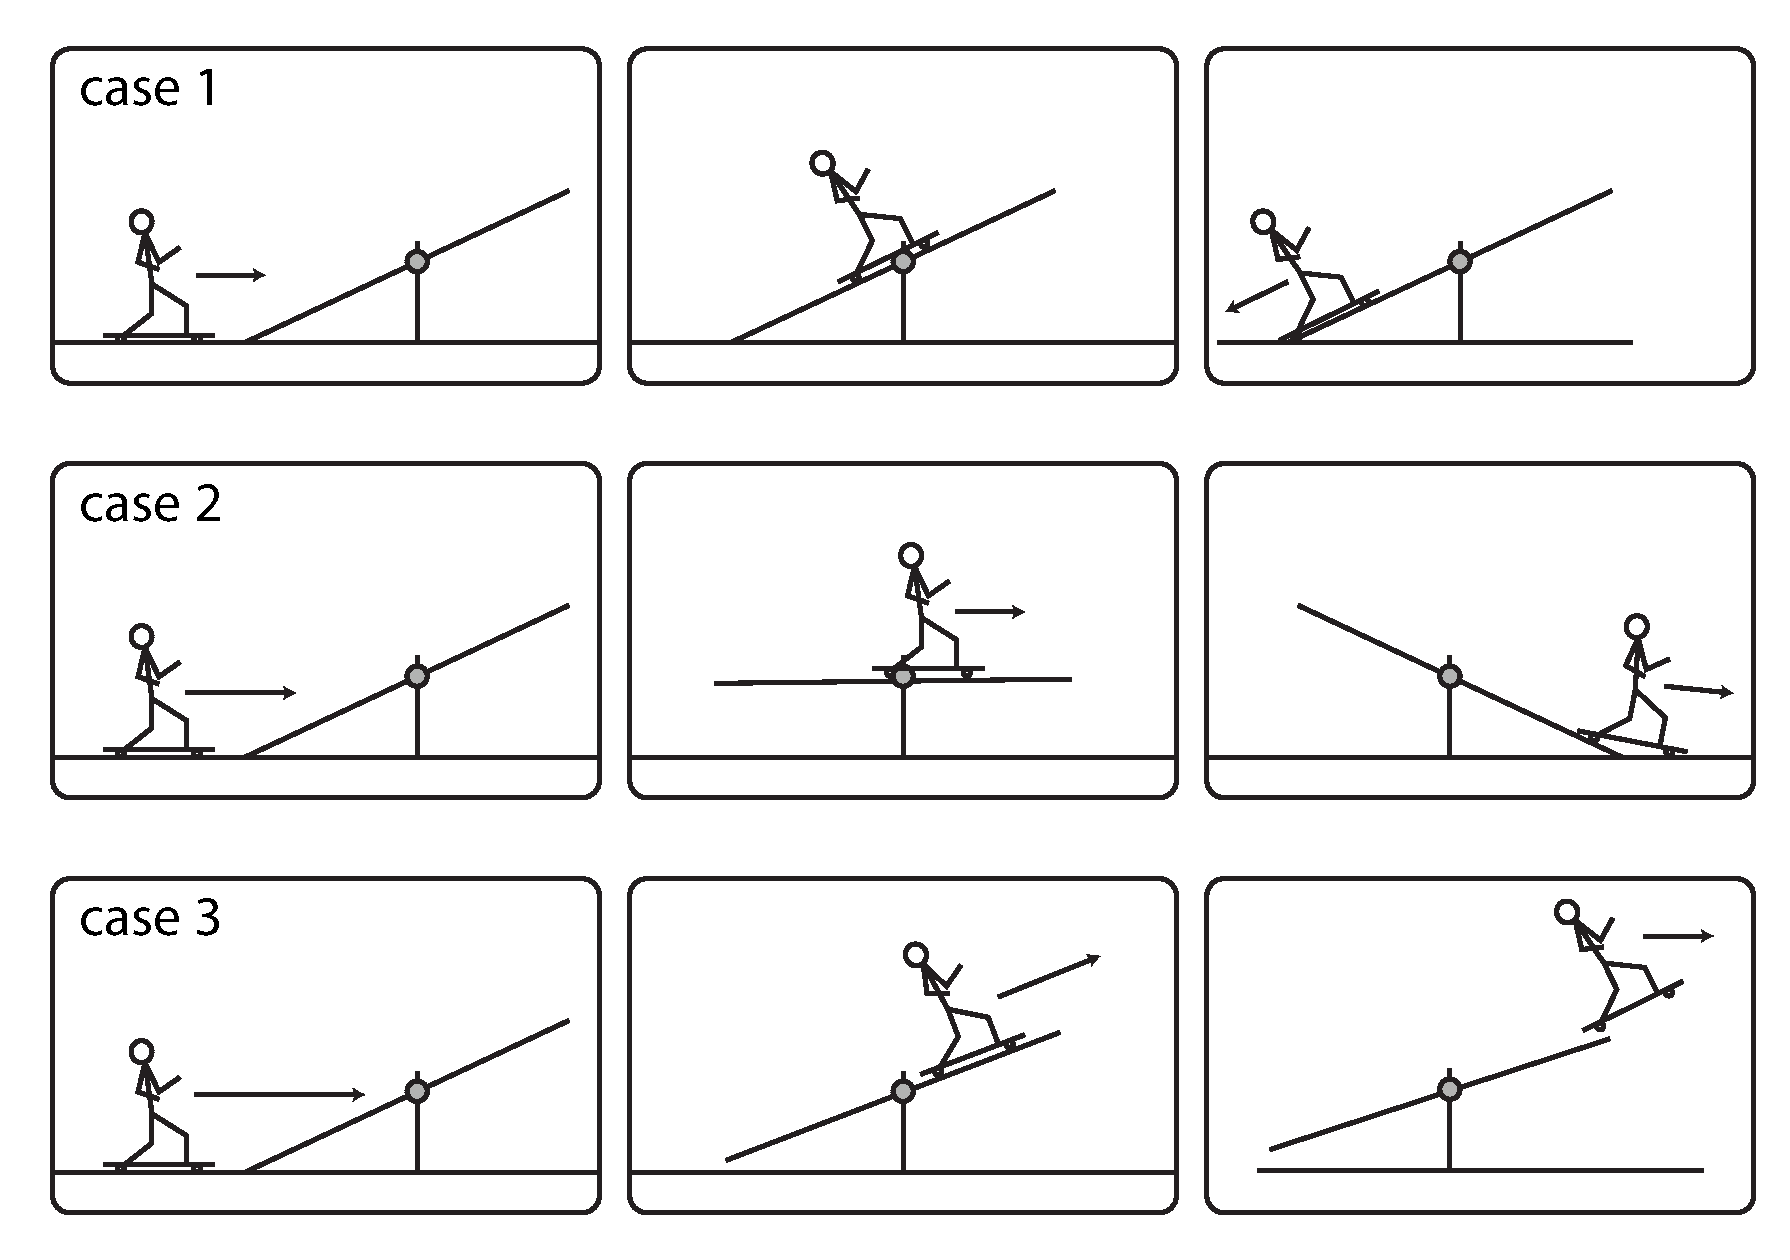
\includegraphics[height=3in]{figs/improvedskateboardkeyframes}

Thinking about the key frames, we can immediately draw some conclusions.  First, it seems pretty clear that the behavior of the system is intimately tied to both where the skateboarder is, and what the orientation of the ramp is.  For example, the further out on the ramp the skateboarder is, the more torque the skateboarder applies to the ramp -- so the skateboarder's position affects how the ramp moves.  By the same token, the ramp's angle will affect the skateboarder -- if it's tilted to the right, the skateboarder will accelerate to the right.  Furthermore, in some situations, it might well be impossible for the system to work.  For example, if the skateboarder weighed far less than the ramp, you could imagine that the skateboarder might either end up going off on the right in midair, or would slide back down and roll off on the left.

Looking at the scenarios outlined above, we can identify a number of different {\it phases} of motion we might want to model:   
\begin{itemize}
\item First, there is the time before the skateboarder goes onto the ramp.  Presumably this is pretty simple -- in fact, we might just want to START at the point when the skateboarder goes onto the ramp. \item The phase during which the skateboarder is on the ramp looks a lot more complex:  the ramp can move (although it's limited by the ground to rotating through a particular angular range), and the skateboarder can move along the ramp.  
\item Finally, there's a phase of motion after the skateboarder leaves the ramp (either by launching off the end of the ramp, or by neatly rolling off on to the ground on either the left or the right side).  This is not so complex, as presumably we don't care how the ramp is moving once the skateboarder leaves the ramp.  It's possible we'd want to think about the launch condition (keyframe 2 above) as distinct from the ``clean'' exit (keyframe 3), but  perhaps it might be enough just to know that the launch takes place.
\end{itemize}

To evaluate this system for competition, it seems like the phase we really need to concentrate on is  motion when the skateboarder is on the ramp.  If we can model this phase, we'll have enough information to say useful things about the system.

\subsection{How many, and what type, of bodies should we consider?}

 During the phase when the rider is on the ramp, it's clear that we care about how both the ramp and the skateboarder move -- so we need at least two parts in this system. 

The ramp's motion is clearly rotational, so weI'll have to use at least a rigid body for that (or, if we wanted to get crazy, a body that can deform).

\begin{marginfigure}
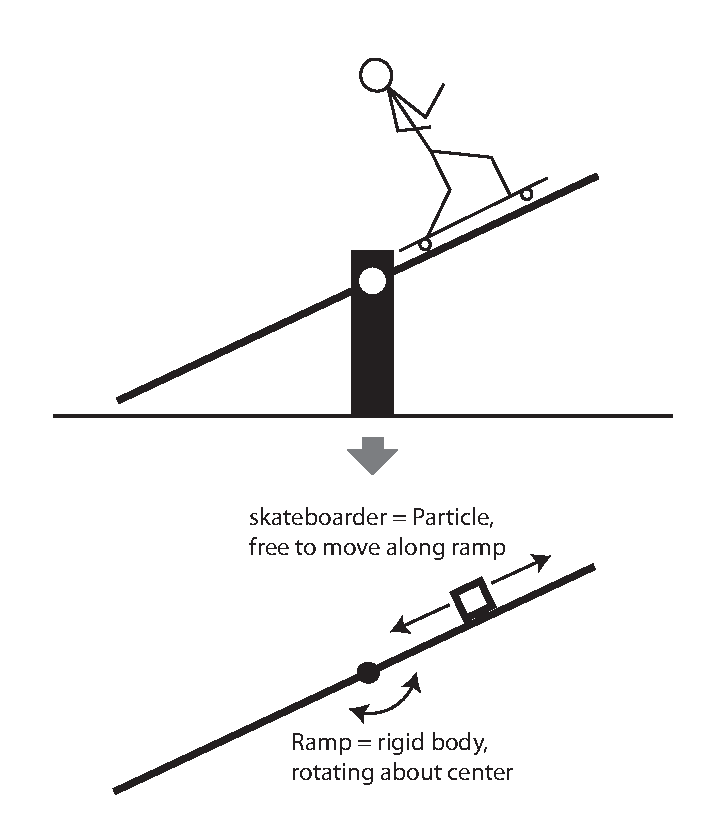
\includegraphics[height=3in]{figs/skateboardabstraction1nocoords}
\caption{Abstraction of skateboarder system to a rigid body and a partlcle}
\end{marginfigure}

The skateboarder could be dealt with in any number of ways - from a particle (i.e., think about the skateboarder as a very compact ``lump'' that slides along the ramp) to a rigid body that slides along the ramp and rotates as the ramp rotates, to a much more complex collection of rigid bodies (e.g., arms, legs, etc.) which are connected to each other in interesting ways (e.g., muscles and joints).


As a first cut (i.e., the easiest approach) we might treat the skateboarder as a particle.  We are ignoring a lot in doing this, but this approach will at least qualitatively capture the behaviors we identified in the key frames.  Naturally we could create a more complex model here -- and maybe we should on a second iteration.



\section{Skateboard Free Body Diagrams}

Since we have identified two different bodies here,  we need two free body diagrams:  one for the skateboarder particle, and one for the ramp rigid body.

We also need to identify what interactions are present:  in what ways does each body interact with the other body, and with the rest of the universe.  A good way to think about this is to imagine ``cutting'' each part of the system out of the rest of the universe, and then thinking about what interactions you had to ``cut'' in order to accomplish this.

For the skateboarder, if we cut him/her out of the universe, we clearly have to cut the gravitational interaction with the earth (i.e., gravity exerts a force on the skateboarder).  We also have to account for the fact that the ramp holds the skateboarder up (i.e., there is a normal force interaction between the skateboarder and the ramp).  It's possible that we'd also want to account for a frictional interaction between the skateboarder and the ramp, but since skateboards typically have pretty good bearings in their wheels, we might also choose to ignore this initially.  And of course, air drag could be important too -- but for the sake of simplicity, we'll leave that out as well.

When we cut the ramp out of the universe, we need only think about what {\it torques} are applied to it -- it's pinned at the center, so the only thing it can do is rotate.  We've already identified a normal force interaction between the ramp and the skateboarder -- i.e., at any given instant, the ramp is pushing up on the skateboarder, and the skateboarder is pushing down on the ramp.  We also could imagine there being a fricitonal torque at the pin -- i.e., the pin might be rusty.  You also might choose to include an ``air drag'' torque on the ramp too: as the ramp rotates through the air, it has to push air out of the way.  But let's ignore these for now, just as we ignored friction in the skateboard -- we can iterate on the model to add these later if we decide it's important.

Thus, we have the following forces and torques that we think will be relevant:

\begin{center}
\begin{tabular}{ p{3cm} | p{5cm} | p{5cm}}
Symbol & Meaning & Dependencies \\
\hline
\hline
$\vec{F}_G$ & Gravitational force acting on the skateboarder & Depends on the skateboarder mass; always points down.\\
\hline
$\vec{F}_N$ & Normal force interaction between sb and ramp -- constrains the skateboard not to fall through the ramp. & Always points normal to the ramp; pushes skateboard up, and ramp down.\\ 
\hline
$\vec{\tau}_N$& Torque exerted by normal force on ramp &  Clearly it directly depends on the position of the skateboard, and on the normal force. \\

\end{tabular}
\end{center}

Finally, having identified the parts of the system as well as the interactions and the relevant symbols, we can draw the free body diagrams:


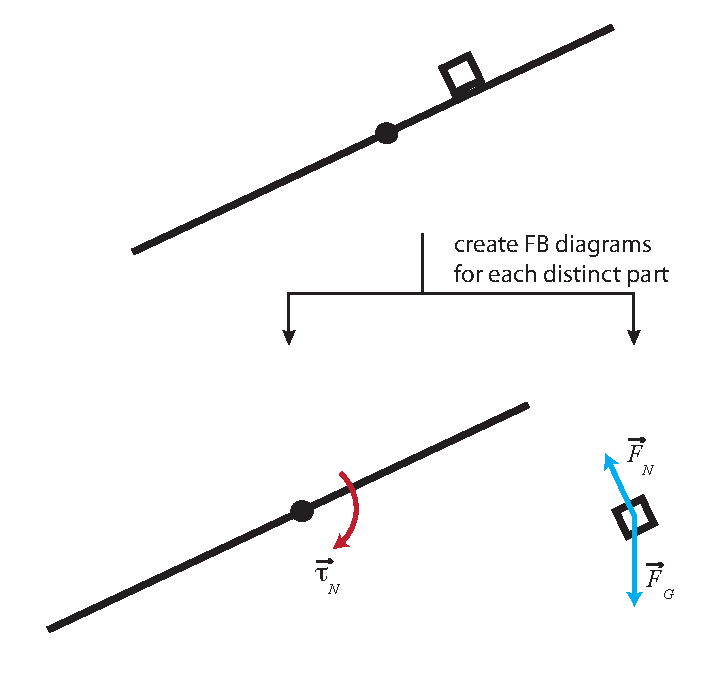
\includegraphics[height=4in]{figs/skateboardfbds}

\section{Quantitative Abstraction: From Free Body Diagrams to Differential Equations}

At this point we've completed our qualitative modeling of the skateboard system.  We've thought through how it might work; we've identified the key behaviors we might want to capture; we've thought about whether to represent different parts of the system as rigid bodies or particles; we've identified the important interactions, and we've drawn a set of free body diagrams.

But in order to develop a dynamical model, we're going to need to get a bit more mathematically formal.  In particular, we need to develop mathematical models for the interactions that we've identified; we need to define state variables and parameters for the system; and we need to combine these definitions into a set of differential equations that describe the motion of the system. 

\subsection{Fundamental and Approximate Mathematical models for interactions}

Objects only move in interesting ways if they are subject to some kind of force or torque -- i.e., if they somehow interact with other objects in the system, or with the rest of the world.  Current models for the universe say that there are a limited number of fundamental interactions that explain every behavior we can observe:
\begin{enumerate}
\item There is the {\it strong force}, which is (not surprisingly) really strong -- but also really short range.  The strong force is pretty much only important within nuclei of atoms.
\item There is the {\it electromagnetic force} , which is both strong and long range.  This is the stuff that holds atoms together, makes light bulbs light up, etc.
\item The {\it weak} force is a short-range force; like the strong interaction, it's pretty much only important within nuclei of atoms.
\item {\it Gravity} is a long-range force, which we tend to know from our daily experience.
\end{enumerate}

However, while virtually every interaction that you can be thought of, ultimately, as a manifestation of either the gravitational force or the electromagnetic force, most of the time we develop {\it phenomenological models} for interactions that don't require keeping track of where every atom is in the system.  For example, when you use Hooke's ``Law'',
$$ F = - k (x-l_0)$$
you are actually using Hooke's {\it model} for how springs behave close to equilibrium.  It's a good model -- but it's not a law. 

\subsection{Gravity and Electromagnetism}
Fundamentally, gravity is an interaction that exists between any two masses:  all masses in the universe attract all other masses.

Newton's law of gravitation (which is, of course, a model),

$$\vec{F}_{12}=\frac{Gm_1m_2}{r_{12}^2}\hat{r}_{12}$$
says 
 that the gravitational force an object \#1 ``feels'' due to object \# 2 ($\vec{F}_{12}$) is proportional (with the universal graviational constant $G$) to the two masses $m_1$ and $m_2$, is inversely proportional to the distance between them squared ($r_{12}^2$), and points from object \#1 towards object \#2 ($\hat{r}_{12}$).  \sidenote{You've possibly not seen the $\hat{r}$ notation before; this notation simply indicates a vector of length 1 and without units in the direction of the vector $\vec{r}$.  It's also commonly used to denote the directions in different coordinate systems -- for example, in the Cartesian coordinate system, $\hat{i}$ denotes a vector of length 1 pointing in the $x$ direction, $\hat{j}$ denotes a vector of length 1 pointing in the $y$ direction, and so forth.}
 
While Newton's law of gravitation is generally applicable, one of the things we frequently do when we're dealing with stuff close to the surface of the earth is to use an alternative gravitational model, 
 $\vec{F} = -mg\hat{j}$.  This model is a simplification of the interaction between the earth and objects near the earth's surface.
 

{\it Can you relate the two gravitational models to each other?  Under what circumstances does $F=-mg$ break down?}

Although gravity is the fundamental force we know best, the reality is that electromagnetic interactions are {\it much} more powerful (about $10^{40} \times$ as powerful, to be specific).  Electromagnetic interactions hold matter together, explain pretty much everything there is to explain about chemistry, and mediate most interactions between different objects -- e.g., gravity keeps you from flying off the earth; electromagnetic forces keep your body from dissolving, and keeps you from sinking into the earth.
 
Although you certainly can use fundamental principles to deal with electromagnetic forces, much of the time it makes more sense to use phenomenological models.  For example, in modeling a spring, we tend to think of it as ``a spring'', not as ``$10^{21}$ atoms arranged in a polycrystalline metal''.  Therefore (and also  due to time and space constraints), we're not going to deal directly with fundamental electromagnetic forces here (e.g., Coulomb's Law, Lorenz Force Law).   You're of course welcome to invoke them if they are relevant for your project.

We also will take a pass on the strong and weak forces -- the models we're developing work well at larger length scales than the nucleus of the atom.
 
 \subsection{Restoring Forces}
Many interactions can be characterized as ``restoring forces'', in the sense that they become larger as you move the system away from an equilibrium configuration, and they are oriented in such a way as to push the system back to equilibrium.  The canonical example of a restoring force is a spring:  springs push back if you compress them, and pull back if you stretch them  -- i.e., the spring force tries to restore the spring to its equilibrium length.  Mathematically, this is expressed as 
$$\vec{F} = - k(l-l_0) \hat{s}$$
where $k$ is the ``spring constant'' (units of N/m), $l$ is the current length of the spring, $l_0$ is the equilibrium length, and $\hat{s}$ is a vector that points outward (towards the object in question) along the spring. Note that this expression says the force will ``push out'' along the spring if the spring is compressed, and will ``pull in'' if the spring is stretched.  

While you might not see all that many springs in daily life, many interactions are well-captured by a spring-like model.  Mathematically, this is true because, if you do a Taylor expansion of the force about equilibrium, the first non-zero term is likely going to be the linear term.  Physically, you can think about many interactions as involving ``springs'' in the form of deformed atomic bonds.  So for many, many situations, a model that says $F=-k\Delta x$, where $\Delta x$ is the displacement from the equilibrium, and the minus sign implies that the force pushes the system back towards equilibrium can be reasonable.

Of course, there are lots of things have what might be called ``one-sided'' springs.  A bungee cord, for example, can stretch -- but if you try to compress it, it simply buckles. 

\subsection{Velocity-dependent forces: Drag, lift, and so forth}
Conceptually, springs and gravitational interactions are both {\it position-dependent} forces:  if you tell me where the parts of the system are located, I can tell you what the forces are.  But there are also a variety of interactions that depend not (just) on where things are, but rather (or also) on how they are moving.

For example, whenever an object moves through a fluid (gas or liquid), there is some loss to the fluid -- there's ``drag''.   While you can certainly develop some pretty complex models for drag, a couple of simple models are commonly employed.  They typically say that (1) the force gets bigger the faster the object moves through the fluid, and (2) the size of the force depends somehow on the nature of the object and on the nature of the fluid.

``Inertial drag'' is usually more appropriate for motion through lower viscosity fluids (e.g., air -- but we're playing fast and loose here).  The inertial drag model says 
$$\vec{F}_{D} = -\frac{1}{2} \rho C_D A v^2 \hat{v}$$
where $\rho$ is the density of the fluid, $C_D$ is the object's ``drag coefficient'' (dimensionless), $A$ is the presented cross-sectional area of the object, $v$ is the object's speed, and $\hat{v}$ is a unit vector in the direction of the object's velocity.  Note that this model does imply that as the speed increases the drag force increases significantly; it also says that the direction of the drag force is always opposite the motion.

``Viscous drag'' is a more appropriate model for motion through more viscous fluids (e.g., molasses); this model says that the drag force is directly proportional to the speed:
$$\vec{F}_{D} = -\beta \vec{v}$$
where $\beta$ is a constant (units of N-sec/m), and $\vec{v}$ is the object's velocity.

Objects moving through fluids can also experience forces in directions that are orthogonal to their velocity: lift, the Magnus force, etc.  We're not going to address these now, but you should be aware of them.

\subsection{Constraint forces: normal contact forces}

In addition to conventional position-dependent and velocity-dependent forces, there are also forces that can be thought of as ``constraint forces'': forces that take on whatever value they need to in order to maintain something about the system.  

The classic example of the constraint force is the so-called ``normal force''.  When you place a book on a table, the interaction between the atoms that make up the book and the atoms that make up the table keep the book from ``falling into'' the table.  
If the book and the table are both stationary, the normal force is simply the opposite of the gravitational force.  But if, for example, you drop the book onto the table the normal force is instantenously much larger -- it ``needs'' to be larger, in order to stop the book from falling into the table.  Similarly, if you lifted up the table, the normal force would become larger as you accelerated the table upwards, because it would ``need'' to be larger in order to keep the book at the position of the table top.  And if you push down on top of the book, the normal force from the table increases to keep the book from falling into the table.  The force ``adjusts'' to enforce the constraint that the matter of the book can't overlap with the matter in the table.

The thing that makes constraint forces tricky is the fact that they are ``whatever they need to be'' in order to maintain the constraint.  They can depend on how every object is moving, what other forces are present in the system, etc.  In comparison, restoring forces, gravitational forces, etc. don't require the object in question to be in any particular place -- they just depend on what the locations or velocities of the various objects are.

Other examples of interactions that are often modeled as constraints include ``tension'' in a string (the force is whatever it needs to be to keep the length of the string less than or equal to the string's maximum length), and ``pin forces'', when you have a pin or axle that connects two objects to each other, but allow them to rotate.  

At a microscopic level, of course, constraint forces are just due to atomic interactions:  the atoms in the rope are bound to each other; the atoms in the table repel the atoms in the book if they get too close.  Given this, sometimes it is sensible to model such interactions not as constraints, but instead as strong restoring forces.  For example, you could certainly think of the normal force as a strong ``spring'' that only acts when the two objects ``clash'' with each other, or you could think of a pin force as a strong spring with zero rest length. This approach has some real advantages, particularly with respect to making the construction of the model simpler and more scalable; on the other hand, this approach can cause numerical issues, as the ``springs'' involved are generally much stiffer than any other springs in the system.

\subsection{Frictional forces: parallel contact forces}
The atomic interactions between two objects also can result in frictional forces -- forces that resist moving one object in parallel with the other object that it is in contact with.  Typically this type of interaction is modeled using ``static'' friction and ``kinetic'' friction.

The model for static friction is a constraint model:  it says that when an object is sitting in stationary contact with another object, there is a certain minimum force required to get that object to move.  If you apply forces below that minimum force (which is proportional to the normal force between the two objects and a coefficient of static friction), the static frictional force resists with just enough to offset the force you apply. So while it is {\it tempting} to say, $F_{static} = \mu_s N$, that's wrong.  It is instead true that $$|F_{static}| < \mu_s N$$
where $\mu_s$ is the coefficient of static friction, and $N$ is the normal force.

Once you ``break'' the stationary contact and the object begins to accelerate, the kinetic frictional force resists the motion.  Unlike static friction, kinetic friction is typically not modeled as a constraint; rather, it is assumed to be a constant force that is proportional to the normal force and a coefficient of kinetic friction:
$$\vec{F}_{kinetic} = - \mu_k N \hat{v}$$
where $\mu_k$ is the coefficient of kinetic friction, $N$ is the normal force, and $\hat{v}$ is the direction the object is sliding along the surface.

{\bf Exercise:}{\it Imagine a coffee cup is sitting on the table.  At $t=0$ I begin to push horizontally on the coffee cup with a force $F$.  Make a plot of the frictional force that the table exerts on the coffee cup as a function of $F$ (how hard I push).}

\section{What about torque?}

Thus far we've only touched on interactions as forces.  Of course, when you are dealing with rotations, it is also important to be able to identify the {\it torques} on the system.  But, since the definition of torque generally depends on the coordinate system, we're going to hold off on that until a little later. 

%\section{What about impulse?}

\section{Coordinate Systems and Parameters}
Once you've made some choices about how you will mathematically model the interactions in the system, you need to introduce a formalism for how you will describe the {\it state} of the system.  

In general, to describe the time-dependent state of a particle, you need to have the following information about it:

\begin{enumerate}
\item You need to know where the particle is.
\item You need to know what the particle's momentum is (or, equivalently, what the particle's velocity is).
\end{enumerate}

\newthought{In the case of rigid bodies}, the list is a bit longer:
\begin{enumerate}
\item You need to know where the center of mass of the body is.
\item You need to know what the body's linear momentum is (or, equivalently, what the velocity of the center of mass is).
\item You need to know what the object's angular position is.
\item You need to know what the body's angular momentum is (or, equivalently, what the angular velocity of object is).
\end{enumerate}

In addition to these {\it state variables}, you also need to know something about the parameters that describe the objects and their interactions-- e.g., the objects' mass,  moments of inertia, drag coefficients, etc.

In order to keep track of the state variables, we need to use a coordinate system to define them.  As a concrete example, let's think about a caber toss: a telephone pole that's been thrown into the air, so that it is both translating (the center of mass is moving) and rotating about its center of mass.  What would we use for a coordinate system?

The most obvious (but not necessarily elegant) coordinate system for particle motion is often the Cartesian coordinate system.  For a particle moving in three dimensions, we choose some fixed point as our origin, set up $x$, $y$, and $z$ axes, and measure the position of the particle using the {\it position vector} $\vec{r}(t)$
$$\vec{r}(t) = x(t) \hat{i} + y(t) \hat{j} + z(t) \hat{k}$$
where $x(t)$, $y(t)$, and $z(t)$ are the time-dependent $x$, $y$, and $z$ positions of the particle, and $\hat{i}$,$\hat{j}$, and $\hat{k}$ are unit vectors in the  $x$, $y$, and $z$ directions.  


If we're dealing with a body that is rotating, we will of course have to define an angle for the rotation (note: we are {\it not} dealing with rotation in three dimensions.  If you're interested in this we can point you towards good sources.).  By convention angles are typically defined as measured counter-clockwise from the $x$ axis.

So, if we think about the caber toss (and just confine ourselves to the $xy$ plane), we get a coordinate system that looks something like this


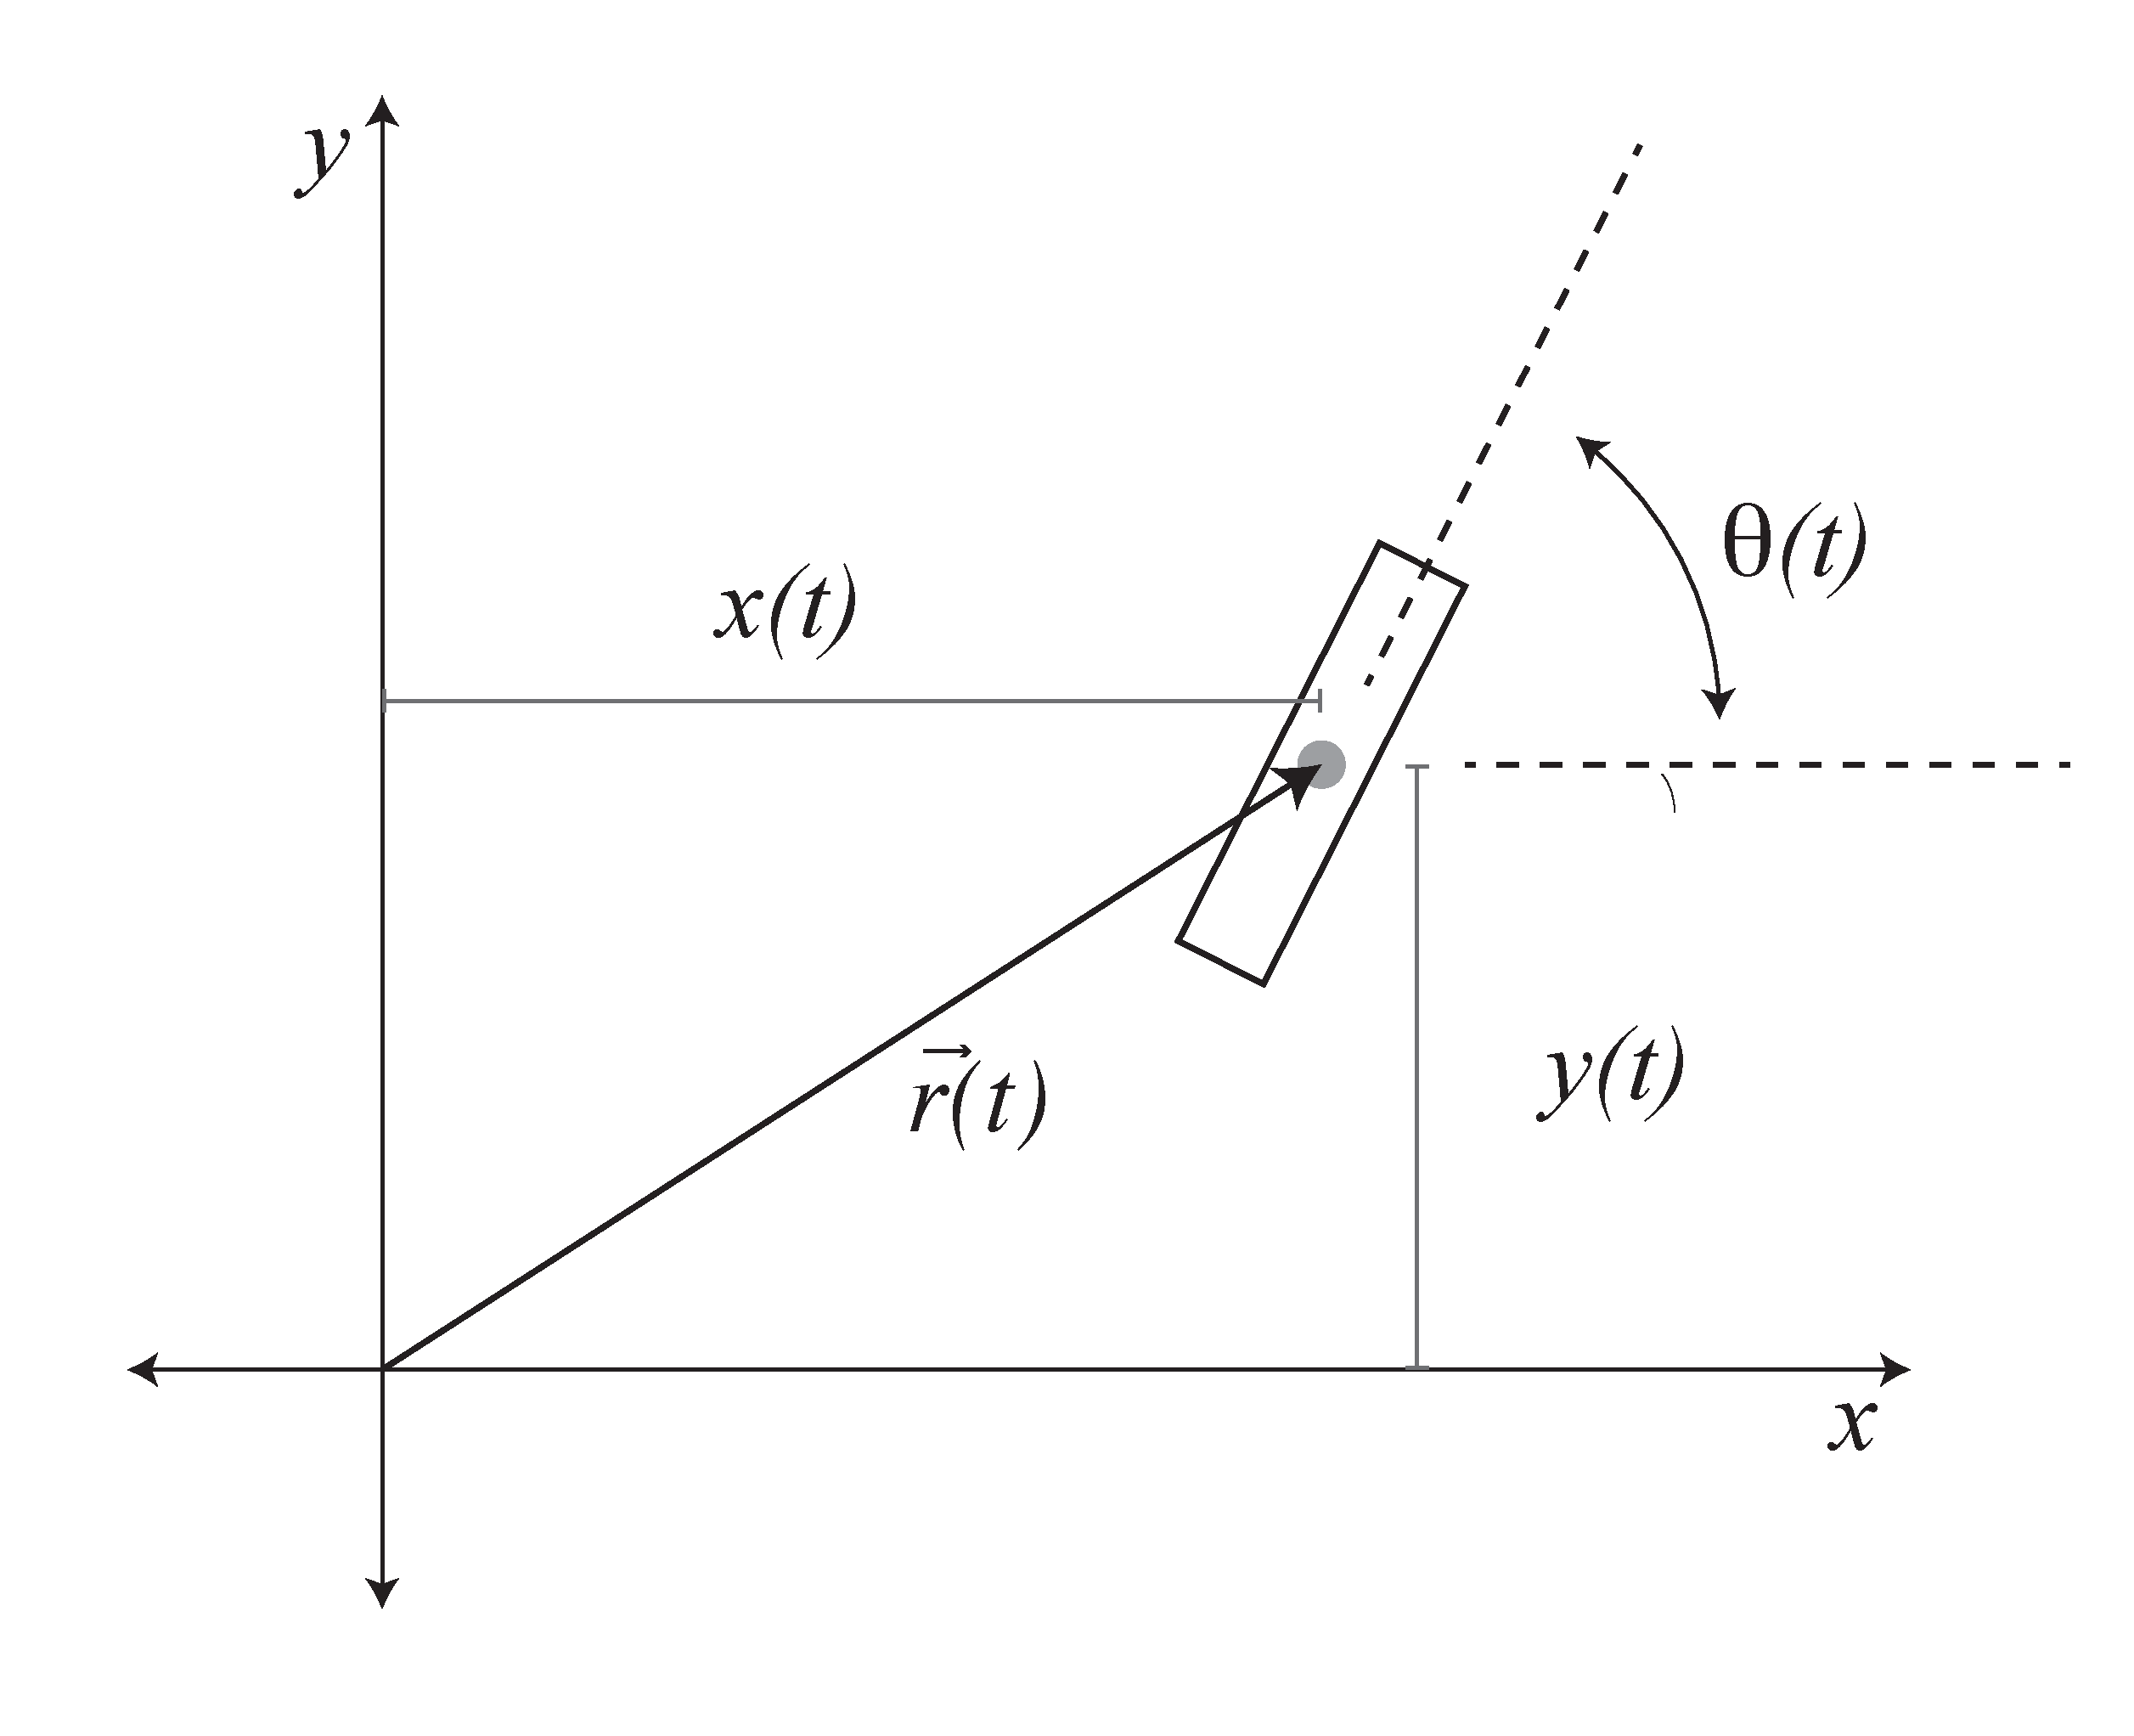
\includegraphics[height=4in]{figs/ExampleCoordSystem}

With this definition of the position and angle, it's pretty easy to figure out what the velocity of the particle is:
$$\vec{v}(t) = \dot{\vec{r}}(t) = \dot{x}(t) \hat{i} + \dot{y}(t) \hat{j} + \dot{z}(t) \hat{k}$$
where $\dot{x}$ denotes the first time derivative of $x$.  

Assuming a mass $m$, we can also determine the linear momentum:$$\vec{p} = m\vec{v}$$

Since we've got an object that is not rotating about the origin, we can either talk about the angular momentum about the object's center of mass:

$$\vec{L}_{com} = I_{com} \omega \hat{k}$$
where $\omega = \dot{\theta}$, or we can talk about the angular momentum about the origin:

$$\vec{L}_{origin} = \vec{r}(t) \times \vec{p}(t) + \vec{L}_{com}$$
Note that this is a {\it cross product} used to determine the angular momentum -- it's not just ``times''!
\section{Determining equations of motion}

We are now at the anti-climactic conclusion of this process:  we've defined momenta, angular momenta, interactions, etc.  All we need to do is apply Newton's second law (and the angular equivalent thereof), which will give us differential equations for linear and angular momentum:
$$\frac{d\vec{p}}{dt} = \sum \vec{F}$$
and
$$\frac{d \vec{L}}{dt} = \sum \vec{\tau}$$

In addition, we of course would like to be able to determine the position, so the kinematic equations give us an additional set of differential equations:
$$\frac{d\vec{r}}{dt} = \vec{v}$$
$$\frac{d\theta}{dt} = \omega$$


These equations {\it look} simple. But it's important to keep in mind that (1) they all depend on each other (e.g., the force often depends on the position which in turn depends on the velocity which finally depends on the force), and (2) each of these equations is a {\it vector} equation -- which means that, in fact, each of these represents two or three separate differential equations:  one for the stuff in the $\hat{i} $ direction, one for stuff in the $\hat{j}$ direction, and so forth. To see how this all works out, let's return to the skateboard example.


\section{An Example of Quantitative Abstraction: The Skateboard Ramp}

When we finished qualitative abstraction of the skateboard ramp, we'd identified a couple of forces (gravity and a normal force) acting on the skateboarder, and a torque acting on the ramp.  Let's take this forward to an actual set of differential equations.

\subsection{Coordinates, state variables, and parameters for the skateboarder}

Before we try to describe the forces, we're going to need to have a coordinate system in place. If we think about the possible states of the system, the ramp can only change its angle -- and this angle is clearly important for describing the state of the system.  The skateboarder, on the other hand, can move up and down the ramp -- but we're assuming that the skateboarder stays in contact with the ramp.  As a consequence, it makes sense to talk about the position of the system being characterized by two state variables:  $r(t)$, the position of the rider along the ramp (measured from the center), and $\theta(t)$, the angle of the ramp (see figure).
\begin{marginfigure}
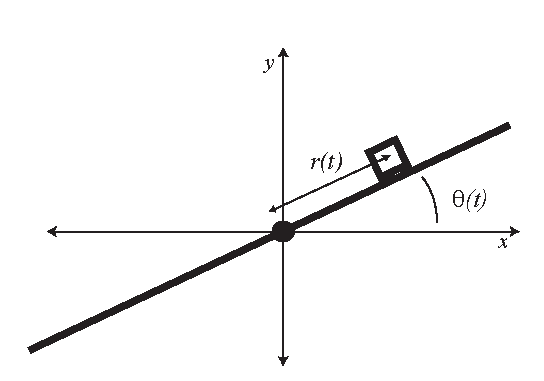
\includegraphics[width=6cm]{figs/SkateboardCoords}
\caption{Proposed coordinate system for the skateboard problem}
\end{marginfigure}

Of course, we will also need to worry about the time derivatives of each of these, as they determine the momenta (which are also state variables).

Note that the number of state variables here s actually LOWER than you might guess it would be by just thinking about a particle and a rotating rigid body.  For a particle, you generally need to know both its position ($\vec{r} = x \hat{i} + y \hat{j}$), and its momentum ($\vec{p} = m(\dot{x} \hat{i} + \dot{y} \hat{j}$) , which gives you four state variables in two dimensions; for the rotating (but not translating) rigid body, you need to know its angular position ($\theta$) and its angular momentum ($\vec{L} = I \omega \hat{k}$).  

However, since the skateboarder is constrained to be on the surface of the ramp, $x$ and $y$ can be expressed purely in terms of how far along the ramp the skateboarder is, and what the angle of the ramp is: $\vec{r} = r \cos \theta \hat{i} + r \sin \theta \hat{j}$.  So, we end up needing two fewer state variables than we might expect otherwise.  This of course  assumes that we are treating the skateboarder as constrained to the ramp -- otherwise we'd need to keep track of the $x$ adn $y$ position of the skateboarder, in addition to the angle of the ramp.

From a parameters perspective, it seems pretty obvious that the mass of the ramp, the mass of the rider, and the length of the ramp will be important.  So, in summary, our state variables and parameters look like this:


\begin{center}
\begin{tabular}{ p{3cm} | p{5cm} | p{5cm}}
State Variable/Parameter & Meaning, range, units, etc. & Why? \\
\hline
\hline
$\theta$ & Angular position of the ramp: runs from some positive angle to some negative angle, depending on ramp design. In radians. & Obvious by inspection. \\
\hline
$\omega$ & Angular velocity of the ramp: radians per second, could in principle be anything & Once the ramp is spinning, it's going to want to keep on spinning \\
\hline
$r$ & Distance of rider from the pivot (positive = to the right of the pivot), in meters & The greater the distance, the greater the torque exerted \\
\hline
$v_r$ & Time rate of change of $r$, in meters per second & Once the rider is moving, the rider wants to keep on moving. \\
\hline
\hline
$m$ & Mass of the rider (kg) &Heavier riders will push down the ramp more.\\
\hline
$L$ & Length of the ramp (m) & Determines both the initial angle and the length of time on the ramp, as well as the ramp's moment of inertia.\\
\hline
$M$ & Mass of the ramp (in kg) & Determines the ramp's moment of inertia -- bigger $M$ means the ramp is harder to move\\

\end{tabular}
\end{center}



\subsection{Mathematical models for skateboarder forces and torques}

We have only a couple of forces to deal with here, so this should be pretty straightforward.
Since we're near the earth's surface, the gravitational force on the skateboarder is  reasonably captured by 
$$\vec{F}_{G} = -m g \hat{j}$$

The normal force is much harder -- given our choices above, it's a constraint force, so about the only thing we can say about it right now is that it is normal to the ramp:

$$\vec{F}_N = N \hat{\theta}$$
where $\hat{\theta}$ is a unit vector that points in the direction of increasing $\theta$ (i.e., normal to the ramp).  We'll have to work through the equations of motion in order to say any more about it.

Finally, the torque on the ramp due to the rider depends on the normal force and on the location of the rider.  If the ramp is pushing up on the rider with a force $N\hat{theta}$, the rider is pushing down on the ramp with a force $-N \hat{\theta}$; this force is acting at the point $r$ along the ramp, which gives us a torque of 
$$\vec{\tau} = -N r \hat{k}$$
Note that this is a negative torque when the normal force and $r$ are positive: when the rider is to the right of the pivot, the ramp wants to rotate clockwise.  This is sensible/

\subsection{Equations of Motion}

We're going to apply the central rules of Newtonian mechanics here:  {\em momentum is conserved, and angular momentum is conserved.}  Mathematically, this means that for ANY system (including parts of a bigger system),
$$\frac{d\vec{p}}{dt} = \sum \vec{F}$$
and
$$\frac{d\vec{L}}{dt} = \sum \vec{\tau}$$
where $\vec{p}$ is the {\it momentum} of the system, $\vec{L}$ is the {\it angular momentum} of the system, $\sum \vec{F}$ is the sum of all the forces being applied to the system, and $\sum \vec{\tau}$ is the sum of all the torques applied to the system.

So let's apply these rules to each part we're dealing with here: the skateboarder, and the ramp.

For the skateboarder, the momentum of the skateboarder is simply the skateboarder's mass times his or her velocity:
$$\vec{p} = m\vec{v}$$
The velocity of the skateboarder requires a little thought.  In general, the velocity is the time derivative of the position. The position is given by 
$$\vec{r} = r \cos \theta \hat{i} + r \sin \theta \hat{j}$$
where $\hat{i}$ is a unit vector in the $x$ direction, and $\hat{j}$ is a unit vector in the $y$ direction.  So, we can find the velocity by taking a time derivative of this.  We of course need to remember the product rule here!
$$\vec{v} = \frac{d\vec{r}}{dt} = (\dot{r} \cos \theta  - r \dot{\theta} \sin{\theta}) \hat{i}+ (\dot{r} \sin \theta + r \dot{\theta} \cos{\theta}) \hat{j}$$

\newthought{Things are going to get ugly} here with all these sines and cosines.  Let's introduce some new notation: $\hat{r}$, which indicates a unit vector pointing along the ramp, and $\hat{\theta}$, which indicates a unit vector normal to the ramp.  If we think through the trig here, we get
$$\hat{r} = \cos \theta \hat{i} + \sin \theta \hat{j}$$
and
$$\hat{\theta} = -\sin \theta \hat{i} + \cos \theta \hat{j}$$
Furthermore, if we think about derivatives here,
$$\frac{d\hat{r}}{dt} = \dot{\theta} \hat{\theta}$$
and 
$$\frac{d\hat{\theta}}{dt} = -\dot{\theta} \hat{r}$$
So then we can write much more neatly:
$$\vec{r} = r \hat{r}$$
and 
$$\vec{v} = \frac{d\vec{r}}{dt} = \dot{r} \hat{r} + r \dot{\theta} \hat{\theta}$$
Ah, isn't that prettier!

We're now ready to apply the law of momentum conservation to the skateboarder.  If we expand the derivative of the momentum (using product rule again on the velocity expression above), we get
$$\frac{d\vec{p}}{dt}  = \frac{d(m\vec{v})}{dt} = m(\ddot{r} \hat{r} + 2\dot{r}\dot{\theta}\hat{\theta} + r\ddot{\theta}\hat{\theta} - r\dot{\theta}^2\hat{r})$$

The righthand side will be the sum of the forces applied to the skateboarder:
$$\sum \vec{F}  = \vec{F}_G + \vec{F}_N$$
So how do we write these out?
Well, $\vec{F}_G = -mg\hat{j}$, which is pretty simple.  Unfortunately, we've written everything in terms of $\hat{\theta}$ and $\hat{r}$, so we need to write $\vec{F}_G$ this way too:
$$\vec{F}_G = -mg\cos \theta \hat{\theta} - mg \sin \theta \hat{r}$$
You'll have to draw yourself a few triangles to convince yourself of this.

$ \vec{F}_N$ is a bit tougher.  By inspection, it will only be in the $\hat{\theta}$ direction.  It's tempting to say also that it has a magnitude that is simply $F_N = mg\cos \theta$.  {\em But this would be very, very wrong!}  Why?  Well, the normal force is a constraint force -- i.e., it is whatever it needs to be to keep the skateboarder from falling through the ramp.  {\em If} the ramp were fixed, $mg\cos \theta$ would be right, because it would end up requiring that the net force was purely in the $\hat{r}$ direction.  But since the ramp is not fixed, it is possible for the skateboarder to accelerate in the $\hat{\theta}$ direction too!  So for now, we'll have to call $F_N$ an unknown quantity.  

Writing out the lefthand and righthand sides for the $\hat{r}$ components, we get the following differential equation:
$$m(\ddot{r} - r \dot{\theta}^2)  = -mg\sin \theta$$
and for the $\hat{\theta}$ components, we obtain
$$m(r\ddot{\theta}  + 2\dot{r}\dot{\theta}) = -mg \cos \theta + F_N$$

\newthought{If we pause and look at these,} in some ways you could say we have two equations and three unknowns: $\ddot{r}$, $\ddot{\theta}$, and $F_N$.  To get our third equation, we need to look at the other chunk in the system: the ramp.

The ramp is a rigid body, which is constrained only to rotate.  This means that the only interesting equation will be the angular momentum equation: the linear momentum of the ramp is ALWAYS zero.  The angular momentum, on the other hand, will only contain a rotational component:
$$\vec{L} = I \dot{\theta} \hat{k}$$
where $I$ is the moment of inertia of the ramp about its pivot, and $\hat{k}$ is a unit vector pointing out of the page (angular momentum points along the axis of rotation).  

Calculating the derivative of this is pretty simple, since both $I$ and $\hat{k}$ don't change in time:  
$$\frac{d\vec{L}}{dt} = I \ddot{\theta} \hat{k}$$

To calculate the RHS of the angular momentum conservation equation, we need to figure out the torque on the ramp.  This is pretty easy too, as the only force that is being applied away from the pivot is the negative of the normal force.  This is being applied perpendicular to the moment arm, so by inspection,
$$\sum \vec{\tau} = \vec{r} \times -\vec{F}_N = -rF_N\hat{k}$$
where $\vec{r}$ is the location of the skateboarder where the normal force is being applied.

Thus our angular momentum conservation equation becomes 
$$I\ddot{\theta} = -rF_N$$

Now we're good to go:  we have three equations, and three things we want to solve for.  Manipulating algebraically, we obtain:
$$F_N = -\frac{ I \ddot{\theta}}{r}$$
and
$$\ddot{\theta} = \frac{-mgr\cos\theta - 2mr\dot{r}\dot{\theta}}{mr^2 + I}$$
and finally 
$$\ddot{r} = -g \sin \theta + r\dot{\theta}^2$$
Whew!

\newthought{Before we go any further,} let's try to see if we can interpret these equations.  Look first at the equation for $\ddot{r}$.  The first term on the RHS side, $-g \sin \theta$,  is a classic ``block on a ramp'' term:  if the ramp is slanted, the block tends to accelerate down the ramp.  The second term, $r\dot{\theta}^2$, is relatively easy to make sense of as well -- if the ramp is spinning at some velocity, the block's speed along the ramp will increase in an outward direction.  For example, imagine a bead on a spinning wire: the bead will get flung off the end of the wire.  This looks like a so-called ``centrifugal force'' (which of course is not a real force, but a result of the fact that the block would have to accelerate in order to stay at a given $r$ on the ramp!).

If we examine $\ddot{\theta}$, there are three things that require interpretation: the two terms in the numerator, and the denominator.  The first term in the numerator, $-mgr\cos\theta$,  looks like the traditional torque due to a gravitational normal force -- pretty easy to buy.  The second term,$- 2mr\dot{r}\dot{\theta}$ , takes some more thought: it says that if the block is moving along the ramp, and the ramp is rotating, there is an additional torque that tends to slow down the ramp.  This takes some thought, but makes sense if you think about it.  Finally, the denominator, $mr^2 + I$, is pretty easy to interpret: it's the total moment of inertia of the system (ramp + skateboarder).

\newthought{Of course, these equations only hold} if the ramp free to move.  Let's think about the other condition...  We'll say that the ramp can rotate between $\theta_{min}$ and $\theta_{max}$.   Then, if $\theta$ drops below $\theta_{min}$, then a couple of thing happen.  First, it seems pretty clear that $\dot{\theta}$ would have to go to zero (i.e., the ramp would stop moving), and it also seems clear that the only way the ramp will start moving again is if $\ddot{\theta}>0$ -- i.e., if the skateboarder is in a location that leads to the ramp getting lifted.  A similar situation applies when $\theta$ gets up to $\theta_{max}$ (although, of course, the condition for the ramp to move here is that $\ddot{\theta}<0$).


\newthought{A final step is to transform} these second order differential equations into a set of first order DE's that will be compatible with an ODE solver. This should be pretty straightforward: we just need to do some relabeling here.

As noted in our state variables, we have $\theta$ and $\omega$, and $r$ and $v_r$.  Clearly two of our DE's are the simple definitional ones:
$$\frac{dr}{dt} = v_r$$
$$\frac{d\theta}{dt} = \omega$$
We obtain our other two DE's for $\omega$ and $v_r$ by substituting these in the equation above:
$$\frac{d\omega}{dt} = \frac{-mgr\cos\theta - 2mr v_r \omega}{mr^2 + I}$$
and finally 
$$\frac{dv_r}{dt} = -g \sin \theta + r\omega^2$$
and now we are ready to simulate!  

\newthought{Maybe we should have done a baseball's flight} as the example problem... Sorry about that.


\end{document}